%% LyX 2.3.2-2 created this file.  For more info, see http://www.lyx.org/.
%% Do not edit unless you really know what you are doing.
\documentclass[english]{upeeei}
\usepackage[latin9]{inputenc}
\usepackage{geometry}
\setcounter{secnumdepth}{3}
\setcounter{tocdepth}{3}
\usepackage[active]{srcltx}
\usepackage{float}
\usepackage{units}
\usepackage{graphicx}

\usepackage{units}
\usepackage{parskip}
\usepackage{graphicx}
%\usepackage{subfigure}
\usepackage{url}  
%\usepackage{stfloats}  
\usepackage{amsmath}   
\usepackage{array}
\usepackage{caption}
\usepackage{afterpage}
\usepackage{textcomp}
\usepackage{lscape}
\usepackage{stfloats}
\usepackage{hyphenat}
\usepackage{makeidx}
\usepackage{amssymb}
\usepackage{hyperref}
\usepackage{hyperref-patches}
%\usepackage{underscore}
\fnbelowfloat
\usepackage{times}
\usepackage{multirow}
%\usepackage{float}
\usepackage{circuitikz}
\usepackage[backend=bibtex,bibstyle=ieee,citestyle=numeric-comp,sorting=none]{biblatex}
\addbibresource{bibliography/chap1.bib}
\usepackage{pgfplots}
%\usepackage{arydshln}
\pgfplotsset{width=7cm,compat=1.5.1}
\renewcommand*{\bibfont}{\small}

\newcolumntype{L}[1]{>{\raggedright\let\newline\\\arraybackslash\hspace{0pt}}m{#1}}
\newcolumntype{C}[1]{>{\centering\let\newline\\\arraybackslash\hspace{0pt}}m{#1}}
\newcolumntype{R}[1]{>{\raggedleft\let\newline\\\arraybackslash\hspace{0pt}}m{#1}}

\newcommand\ddfrac[2]{\frac{\displaystyle #1}{\displaystyle #2}}
\pgfplotsset{compat=1.14}

\makeatletter

%%%%%%%%%%%%%%%%%%%%%%%%%%%%%% LyX specific LaTeX commands.
\providecommand{\LyX}{L\kern-.1667em\lower.25em\hbox{Y}\kern-.125emX\@}
%% Because html converters don't know tabularnewline
\providecommand{\tabularnewline}{\\}

\@ifundefined{showcaptionsetup}{}{%
 \PassOptionsToPackage{caption=false}{subfig}}
\usepackage{subfig}
\makeatother

\usepackage{babel}

\begin{document}
%%% UP EEEI undergraduate project template
%% v0.1 by Louis P. Alarcon 11/22/2011
%%
%% LyX template - use with the following files:
%% 	uct10_new.clo, uct11_new.clo, uct12_new.clo, upeeei.cls, upeeei.layout
%%

%% Place project title here
\title{Evaluation of Performance Parameters of Star and Partial Mesh Topology by Designing an Indoor Air Quality Monitoring (IAQM) System based on IoT for COVID-19 Application} 

%%
%% Author information

\author{
Jean Francois Thomas Berin\\ 2019-05739\\ \emph{BS Electronics Engineering} \\ \\
Dennis Salvador Valeza Ignacio\\ 2019-02486\\ \emph{BS Computer Engineering} \\ \\
Stephen Nap Saroca\\ 2019-05797\\ \emph{BS Electronics Engineering}
}

%%
%% Month and year of submission/graduation
\degreeyear{2023} 
\degreesemester{January} 

% Put your advisers here:
\chair{Jaybie A. de Guzman}
\othermembers{\ \\ \ } 
\numberofmembers{3}

\field{Electrical/Computer/Electronics and Communications Engineering} 
\campus{Diliman} 

\maketitle

% uncomment the following four lines once you need to submit your approved 198/199 manuscript after the final assessment
\newgeometry{verbose,tmargin=0.5in,bmargin=1in,lmargin=0.5in,rmargin=0.5in}
%\newpage
\thispagestyle{empty}

\noindent \begin{center}
\begin{tabular}{c}

\includegraphics[width=0.625in]{EEE Documentation/198_199_frontmatter/UP_logo_maroon.jpg}\tabularnewline
UNIVERSITY OF THE PHILIPPINES\tabularnewline
\end{tabular}
\par\end{center}

\vspace*{\fill}

% replace [Course] with specific course
\begin{center}
Bachelor of Science in [Course] Engineering
\par\end{center}

\vspace*{\fill}

% student names
\begin{center}
[Student/s Name]\\\par
[Student/s Name]\\\par
%[Student/s Name]\\\par
\end{center}

% project title
\begin{center}
[Project Title]
\par\end{center}

\vspace*{\fill}

\begin{center}
Undergraduate Project Adviser:\\\par
\par\end{center}

% adviser/s
\begin{center}
[Adviser/s Name]\\\par
[Adviser/s Name]\\\par
%[Adviser/s Name]\\\par
\end{center}

\begin{center}
Electrical and Electronics Engineering Institute \\\par
University of the Philippines Diliman
\par\end{center}

\vspace*{\fill}

\begin{center}
Undergraduate Project Reader:\\\par
\par\end{center}

\begin{center}
[Examiner/s Name] 
\par\end{center}

\begin{center}
Electrical and Electronics Engineering Institute \\\par
University of the Philippines Diliman 
\par\end{center}

\vspace*{\fill}

\begin{center}
Date of Submission 
\par\end{center}

\begin{center}
[Date of Final Manuscript submission]
\par\end{center}

\vspace*{\fill}

\begin{center}
Permission is given for the following people to have access to this thesis: 
\\\par\end{center}

\noindent \begin{center}
\begin{tabular}{|l|c|}
\cline{1-1} 
Circle one or more concerns: \hspace*{1cm}I\qquad{}P\qquad{} C & \multicolumn{1}{c}{}\tabularnewline
\hline 
Available to the general public & Yes/No\tabularnewline
\hline 
Available only after consultation with author/thesis adviser & Yes/No\tabularnewline
\hline 
Available only to those bound by confidentiality agreement & Yes/No\tabularnewline
\hline 
\multicolumn{1}{l}{\hspace*{10cm}} & \multicolumn{1}{c}{\hspace*{2cm}}\tabularnewline
\end{tabular}
\par\end{center}

Students\textquoteright{} signature/s: \\

Signature/s of undergraduate project advisers:
%% Note: You may decrease the amount of vertical spacing indicated in \vspace*{} in the case that you need to include more than three advisers.
\chapter*{Approval Sheet}
\thispagestyle{empty}
% Replace [Project Title] and [Student Name/s] with project title and student name/s respectively
In partial fulfillment of the requirements for the degree of [Course], this project
entitled ``[Project Title]'', prepared and submitted by [Student Name/s], is hereby recommended for approval.

\vspace*{1cm}

% replace [Adviser Name] with adviser name
\begin{tabular}{llc}
 &  & \tabularnewline
\cline{1-1} \cline{3-3} 
[Adviser Name 1] &  & Date\tabularnewline
Adviser &  & \tabularnewline
 &  & \tabularnewline
 
% uncomment the following lines for a second adviser
% &  & \tabularnewline
%\cline{1-1} \cline{3-3} 
%[Adviser Name 2] &  & Date\tabularnewline
%Adviser &  & \tabularnewline
% &  & \tabularnewline
 
% uncomment the following lines for a third adviser
% &  & \tabularnewline
%\cline{1-1} \cline{3-3} 
%[Adviser Name 3] &  & Date\tabularnewline
%Adviser &  & \tabularnewline
% &  & \tabularnewline
 
\hspace*{10cm} & \hspace*{1cm} & \hspace*{2cm}\tabularnewline
\end{tabular}

\vspace*{1cm}

% replace [Course] with course name
\noindent Accepted in partial fulfillment of the requirements for
the degree of [Course].

\vspace*{1cm}
% replace [Panel Member/s Name] and [Institute Director Name] with examiner name and the name of the institute director respectively
\begin{tabular}{llc}
 &  & \tabularnewline
\cline{1-1} \cline{3-3} 
[Panel Member/s Name] &  & Date\tabularnewline
Panel Member &  & \tabularnewline
 &  & \tabularnewline
\hspace*{10cm} & \hspace*{1cm} & \hspace*{2cm}\tabularnewline
 &  & \tabularnewline
\cline{1-1} \cline{3-3} 
[Institute Director Name] &  & Date\tabularnewline
Director, Electrical and Electronics Engineering Institute &  & \tabularnewline
\end{tabular}

%\newpage
\chapter*{University Permission Page}
\thispagestyle{empty}


I hereby grant the University of the Philippines non-exclusive worldwide,
royalty-free license to reproduce, publish, and public distribute
copies of this work in any form subject to the provisions of applicable
laws, the provisions of the UP IPR policy and any contractual obligations,
as well as more specific permission marking on the Title Page.\\

\noindent Specifically I grant the following rights to the University:
\begin{itemize}
\item to upload a copy of the work in the theses database of the college/school/institute/department
and in any other databases available on the public internet; 
\item to publish the work in the college/school/institute/department journal,
both in print and electronic or digital format and online; and 
\item to give open access to above-mentioned work, thus allowing \textquotedblleft fair-use\textquotedblright{}
of the work in accordance with the provisions of the Intellectual
Property Code of the Philippines (Republic Act No. 8293), especially
for teaching, scholarly, and research purposes. 
\end{itemize}
\vspace*{2cm}

\begin{tabular}{llc}
 &  & \tabularnewline
\cline{1-1} \cline{3-3} 
[Student Name/s and Signature] &  & Date\tabularnewline
 &  & \tabularnewline
 &  & \tabularnewline
 
% &  & \tabularnewline
%\cline{1-1} \cline{3-3} 
%[Student Name/s and Signature] &  & Date\tabularnewline
% &  & \tabularnewline
% &  & \tabularnewline

% &  & \tabularnewline
%\cline{1-1} \cline{3-3} 
%[Student Name/s and Signature] &  & Date\tabularnewline
% &  & \tabularnewline
% &  & \tabularnewline

 \hspace*{10cm} & \hspace*{1cm} & \hspace*{2cm}
\end{tabular}

%\newpage
\chapter*{Acknowledgment}
\thispagestyle{empty}

Insert acknowledgement message here\\

[Name]

[Student Number]

[Course]

\restoregeometry

\begin{abstract} 

%Your abstract goes here...
The COVID-19 pandemic caused by the SARS-CoV-2 virus has induced the increase of time spent indoors by the general population.  The disease is transmitted through the inhalation of droplets and small particles in the air containing the virus.  With regards to this, poor indoor air quality has been discovered to influence higher infection rates of the disease in humans.  Indoor air quality monitoring (IAQM) systems employing Internet-of-Things (IoT) technology have emerged to aid in the detection of indoor air pollution (IAP).  However, most of these existing systems do not account for COVID-19 parameters and have issues regarding data transmission and power management.  This project consists of a real-time IoT-based IAQM system capable of monitoring air quality parameters related to COVID-19.  The sensors used are the Nova PM sensor SDS011, MQ135, and DHT22 which will be integrated to ESP32, a microcontroller unit, to create a sensor node.  The sensor nodes of the system measure specific air quality parameters which are PM2.5, PM10, carbon monoxide (CO), temperature, and relative humidity.  The sensor nodes are connected to a gateway by using the star or partial mesh topology for comparison.  Then, the data acquired by the gateway is sent to a Blynk database server for data visualization, monitoring, and analysis.  Throughput, latency, packet loss, power consumption, and mean time between failure (MTBF) were measured to evaluate the IAQM system.  For further testing, the number of sensor nodes were varied to analyze its impact on the performance of the system.  The outcome of this project could benefit the educational community as there is already an ongoing transition from online classes to face-to-face setup while still in the COVID-19 pandemic.

\abstractsignature\end{abstract}

\begin{frontmatter} 
\setlength{\parskip}{0pt}
\tableofcontents{}
\listoffigures
\listoftables
\end{frontmatter} 

\def\MASTERDOC{true}
\cleardoublepage{}
\chapter{Introduction\label{cha:Introduction}}

\section{COVID-19 and its Relevance to Air Quality}
\label{section:sec01_01}

The COVID-19 pandemic caused by the contagious SARS-CoV-2 virus which severely affects the human respiratory system, triggered a disruption in most of the world?s economy for tourism and retail and forced the implementation of stringent containment measures \cite{RePEc:imf:imfwpa:2021/018}. The COVID-19 disease gets transmitted when people breathe air contaminated by droplets and small airborne particles containing the virus. The risk of breathing the disease is highest when people are in close proximity.  It is then crucial to maintain a considerable distance from others and for people to stay most of the time inside their homes. Unfortunately, they can also be inhaled over longer distances, even when indoors  \cite{https://doi.org/10.1111/ina.12751}
\cite{doi:10.1126/science.abd9149}.

During the pandemic, governments all around the world restricted the movement of the general population through the process of self-quarantining indoors.  This led to the increase in the amount of time people stayed indoors, thus indoor air pollution (IAP) worsened during the COVID-19 lockdown \cite{Du_2020}.  Many studies confirm that indoor air is more deadly than outdoor air \cite{Cincinelli} [6].

\cleardoublepage{}

\chapter{Related Work\label{cha:RRW}}

This chapter details the different works \textbf{related} to your topic. The rule of thumb in writing this section is to start from a broad range of topics and narrowing it down to your topic of interest.

Note that this is a \emph{review} so you need to identify the \emph{problems} of the work you are reviewing. Critically criticize their work, identify what is common between them and differentiate your proposed solution from them. This is the most difficult part of your proposal.

\section{Section 2-1}
\label{section:sec02_01}

\section{Section 2-2}
\label{section:sec02_02}

\cleardoublepage{}




\chapter{Problem Statement and Objectives \label{cha:ProbStatement}}

\section{Problem Statement}

The problem is stated here in one coherent paragraph summarizing your RRW.

\section{Objectives of the Project}
\label{section:sec_obj}
The \textbf{concrete} goals of the project are stated here. Define the metrics that will measure the success of your project. It will be the basis for your examiner for your 198 grade.

\section{Scopes and Limitations}
\label{scopes}
This optional section defines the scope of the project. The project must be doable in 16 weeks and this section ensures that limit to be possible for you. The stated goals from section \ref{section:sec_obj} may not be achievable within 16 weeks if you don't define the scope.

\cleardoublepage{}



\chapter{Methodology\label{cha:Methodology}}

This chapter outlines the different design and testing techniques you will perform to measure the success of your project. For the designs, detail everything up to the calculations and derivations. Cite your references if possible. Include relevant block diagrams and/or graphs. For the experiments, detail everything down to the number of trials, parameters you will measure, and the number of data points you will measure.

\section{Displaying an Image using includegraphics}

\begin{figure} [H]
    \centering
    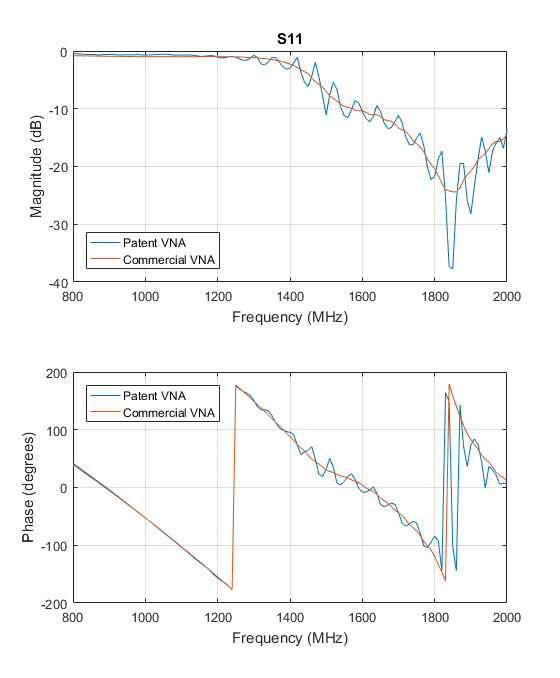
\includegraphics[scale=0.5]{figures/S11_hpf.png}
    \caption{This figure is a graph}
    \label{fig:S11_graph}
\end{figure}

Figure \ref{fig:S11_graph} is an example of an image that is inserted using \texttt{includegraphics\{\}} command. The command can use a JPEG, PNG, and GIF file extensions to place an image. The \texttt{figure} float object needs the \texttt{H} in the command seen above to determine how it will be placed. Table \ref{tab:float_placement_identifier} summarizes the different float object placement commands.

\begin{table}[!t]
    \centering
    \begin{tabular}{|c|c|}
        \hline
        \textbf{Command} & \textbf{Effect} \\\hline
        h & Place the float \emph{here}, i.e., \emph{approximately}\\
         & at the same point (however, not \emph{exactly} at the spot) \\\hline
        t & Place the float at the \emph{top} of the page \\\hline
        b & Place the float at the \emph{bottom} of the page \\\hline
        p & Put on a special \emph{page} for floats \\\hline
        ! & Override internal parameters LaTeX uses for\\
         & determining "good" float positions \\\hline
        H & Places the float at precisely the location in the LaTeX code.\\
         & Requires the \texttt{float} package, i.e., \texttt{usepackage{float}} \\\hline
    \end{tabular}
    \caption{Floating object placement identifier}
    \label{tab:float_placement_identifier}
\end{table}

\section{Generating an Image using circuitikz}

\begin{figure} [H]
    \centering
    \begin{circuitikz} [american voltages, american currents, scale=0.8]
        \draw [thick]
            (0,0) node[op amp] (opamp) {}
            (-1.5,0.625) -- (-2.5,0.625) -- (-2.5,2) to[R,l=$1\,M\Omega$] (2,2) -- (2,0) -- (1.5,0)
            (-2.5,2) to [R,*-,l_=$100\,k\Omega$] (-5.5,2) node[ground]{}
            (-1.5,-0.625) to[short,-o] (-2.5,-0.625) node[label={left:$v_i$}]{}
            (2,0) to[short,*-o] (3,0) node[label={right:$v_o$}]{}
            
        ;
    \end{circuitikz}
    \caption{This is an operational amplifier circuit}
    \label{fig:op_amp}
\end{figure}

Figure \ref{fig:op_amp} is an example of an image generated through the TikZ package of LaTeX. Specifically, it uses the CircuiTikZ package which is specialized for circuit diagrams. It is by no means limited to circuits as block diagrams can also be generated using the said package \cite{circuitikz_howto,tikz_howto}. Just consult the circuitikz and tikz manuals on how to use the package.

\section{Generating a Table}

The code below is used to make table \ref{tab:AM_comparison}. The \texttt{tabular} command is used to generate the table. The command \texttt{hline} generates the \emph{horizontal lines} between rows. The lines between columns are generated automatically.

\begin{table}[H]
    \centering
    \begin{tabular}{|c|c|}
        \hline
        \textbf{Modulation Type} & Description \\\hline
        Full AM & Loren ipsum dolor... \\\hline
        DSB-SC & Loren ipsum dolor... \\\hline
        SSB & Loren ipsum dolor... \\\hline
        VSB & Loren ipsum dolor... \\\hline
        VSB+C & Loren ipsum dolor... \\\hline
    \end{tabular}
    \caption{Summary of Amplitude Modulation Schemes}
    \label{tab:AM_comparison}
\end{table}{}

\section{Making a Citation}

The \texttt{cite} command is used to make citations that are taken from \texttt{bibfile.bib} seen in the files of the LaTeX manuscript. An online manual can be used to check the supported formats of the IEEE format bibliography \cite{bibtex_howto}. If a citation is taken from the IEEEXplore Digital Library, the BibTeX format can be easily downloaded as shown in figures \ref{fig:IEEEXplore_citation} and \ref{fig:IEEEXplore_BibTeX}. The citation will automatically appear in the bibliography section of the document \cite{quitevis_ambatali}.

\begin{figure} [H]
    \centering
    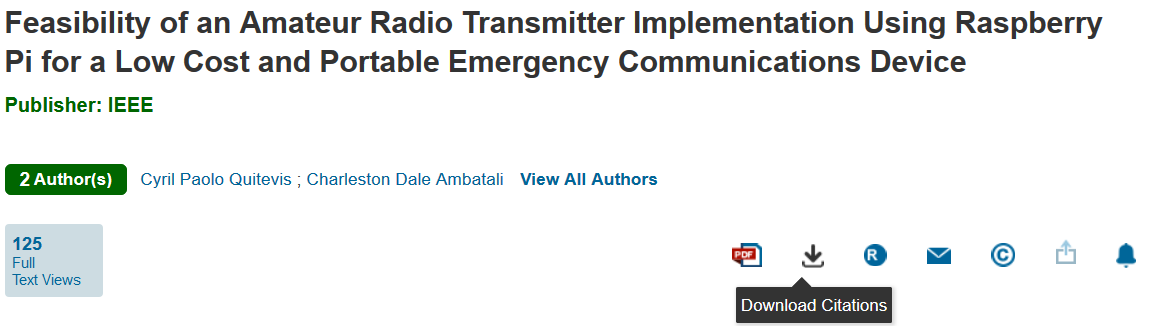
\includegraphics[scale=0.5]{figures/download_citations.png}
    \caption{IEEEXplore Article Page}
    \label{fig:IEEEXplore_citation}
\end{figure}

\begin{figure} [H]
    \centering
    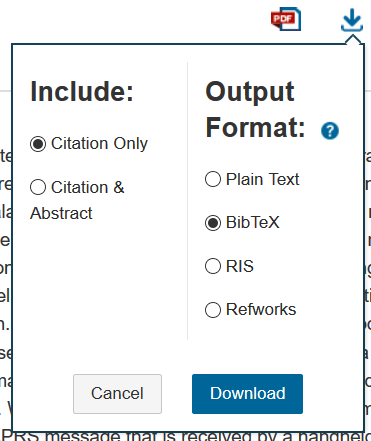
\includegraphics{figures/download_bibtex.png}
    \caption{IEEEXplore Download BibTeX}
    \label{fig:IEEEXplore_BibTeX}
\end{figure}

\cleardoublepage{}




\chapter{Preliminary Findings\label{cha:Prelims}}

This is an \emph{optional} chapter that reports on the feasibility of your project. You may be required by your adviser to have a preliminary work ready by the end of the semester.

\cleardoublepage{}




\chapter{Project Schedule and Deliverables\label{cha:Project-Sked}}


\section{Gantt Chart }

A Gantt Chart detailing the different steps to complete your project. Try to cram as much detail into this chart as possible and also show a clear division of tasks if you will work on a project as a group.

\section{Halfway-point Deliverables}

Define the expected output upon halfway of the semester, i.e., at the end of 8 weeks. This will aid your examiner and adviser on determining if you should still continue your 198 or fail you pre-emptively.

\cleardoublepage{}

\printbibliography


\end{document}